% class
%\documentclass{llncs}
%\input glyphtounicode\pdfgentounicode=1
%% packages
%%\usepackage[colorinlistoftodos]{todonotes} % for comments
%%\usepackage{soul} % strikethrough
%\usepackage{amsmath}                % math package
%\usepackage{float}                  % float package
%\usepackage[caption=false]{subfig}  % caption option on package
%\usepackage{graphicx}               % figure package
%\usepackage{epstopdf}               % eps to pdf conversion
%\epstopdfsetup{update}            
%\usepackage[perpage]{footmisc}      % change numbering of footnotes
%\usepackage{nicefrac}               % allow better in-line fractions a/b
%\usepackage{multirow,bigdelim}       % multiple rows in tables
%\usepackage{booktabs}               % for tabs
%\usepackage{nicefrac}
%\usepackage{bm}
%\usepackage{multirow}
%\usepackage{colortbl}
%\usepackage{subfig}
%% \usepackage[subtle, title=normal, bibliography=normal]{savetrees24}
%\pdfinfo{
%  /Title (Multitask learning)
%  /Creator (*)
%  /Producer ()
%  /Author (*)
%  /Subject (*)
%  /Keywords (*)
%}

\chapter{Part I: Uncertainty in Multitask Learning}
\label{chapter:multitaskuncertainty_part1}

\textcolor{red}{Here I could use my work with ThinkSono to motivate the importance of tuning the relative weightings of task losses to benefit from multi-task learning \cite{tanno2018autodvt}.}

Multi-task neural network architectures provide a learning mechanism that jointly synthesises information from distinct sources. The success of multi-task learning stems from inductive transfer, which is known to improve the performance of a model by learning task-invariant representations. Multi-task learning is ideal in the context of MR-only radiotherapy planning as it can jointly synthesize a synthetic CT (synCT) scan (regression) and an automated contour of organs-at-risk (segmentation) from MRI data. We propose to use a probabilistic deep-learning formulation to estimate the \textit{intrinsic} and \textit{parameter} uncertainty through a heteroscedastic noise model, where parameter uncertainty is modelled using approximate Bayesian inference. This allows the sampling of multiple segmentations and synCTs that share their network representation, enabling a fully end-to-end uncertainty aware MRI-based probabilistic planning system. We show that our model produces more accurate and consistent synCTs with a better estimation in the variance of the errors, equivalent state of the art results in OAR segmentation and a methodology for quality assurance in treatment planning. The model also produces samples with anatomically-consistent segmentations and synCTs, a necessary characteristic in probabilistic planning models. 

\section{Introduction}
% (version 2):
The state-of-the-art in radiotherapy treatment planning requires acquiring a magnetic resonance (MR) scan to accurately segment the target and surrounding organs-at-risk (OARs), and a registered computed tomography (CT) scan to inform the photon attenuation. This approach has seen limited translation to clinical practice as extensive data acquisition is time-consuming and modality registration may introduce unacceptable errors that propagate in the planning process. MR-only treatment planning has been proposed as a solution to these issues and involves the generation of a synthetic CT (synCT) scan from the MR scan. This deterministic synthesis process, when combined with a hand drawn region of interest and a set of safety margins, provides a deterministic radiotherapy plan that is intrinsically dependent on the quality of the inputs. On the other side, probabilistic planning systems allow the implicit estimation of dose delivery uncertainty through a Monte Carlo sampling scheme. A system that can sample possible synCT and OAR segmentations would enable the development of a fully end-to-end uncertainty-aware probabilistic planning system.  

Classical methods for simulating a synCT and segmenting corresponding MR scans have originated from multi-atlas propagation \cite{ninon2017}. Recently, applications of convolutional neural networks (CNNs) to CT synthesis from MRI have become a topic of growing interest due to their reconstruction performance. To alleviate the problem of missing high-frequency information in synCT due to mean-squared reconstruction loss, Nie et al. \cite{nie2017} employed a conditional generative adversarial network to capture fine texture details whilst Wolterink et al. \cite{wolterink2017} extended this idea using a CycleGAN to leverage the abundance of unpaired training sets of CT and MR scans. However, despite this advancement, all of these methods commit to a single prediction, with no measure of confidence. The lack of uncertainty information limits utility in view of current and future probabilistic dose delivery systems. Also, knowing the variance of the predictions would enable the development of quality assurance systems, improving the safety of such a system. Finally, none of the CNN-based methods segment OARs, and if a model was trained to do so, it would not produce OAR segmentations and synCT results that are consistent, which is necessary in radiotherapy planning.

Kendall et al.\cite{kendall2017multi} recently devised a method for uncertainty modelling, showing its value in multi-task learning problems. However, this model assumes homoscedastic (constant) noise in the task output, which is unrealistic for most imaging data and yields non-meaningful measures of predictive uncertainty in a regression task. Tanno et al. \cite{tanno2017bayesian} and Kendall et al. \cite{kendall2017uncertainties} raised the importance of modelling both \textit{intrinsic} and \textit{parameter} uncertainty to build more robust predictive models for medical image analysis and computer vision. The former describes noise inherent in the observations whilst the latter quantifies the degree of ambiguity in the model parameters given the observed data. 

This paper makes use of \cite{tanno2017bayesian} to enrich the probabilistic multi-task learning method proposed in \cite{kendall2017multi}, enabling modelling of the spatial variation of intrinsic uncertainty via heteroscedastic noise, and integrating parameter uncertainty via dropout. We thus propose a probabilistic dual-task network, which operates on a MR image and simultaneously provides three valuable outputs necessary for probabilistic radio-therapy planning: (1) generation of syncCT; (2) segmentation of the OARs; (3) quantification of predictive uncertainty in (1) and (2). The proposed architecture integrates the methods of uncertainty modeling in CNNs \cite{tanno2017bayesian,kendall2017uncertainties} into a multi-task learning framework with hard-parameter sharing, in which the initial few layers of the network are shared across the two tasks (synthesis and segmentation) and branch out into task-specific layers (Fig.\ref{fig:diagram}). This probabilistic formulation not only provides an estimate of uncertainty over predictions from which one can stochastically sample the space of solutions, but also naturally confers a mechanism to automatically select the relative weighting of task losses, in contrast with prior work which relied on uniform or hand-tuned weighting \cite{moeskops2016deep}.  

\section{Methods}
We propose a probabilistic dual-task CNN-based algorithm which takes an MRI image, and simultaneously estimates the distribution over the corresponding CT image and the segmentation probability of the OARs. We use a heteroscedastic noise model and binary dropout to account for \textit{intrinsic} and \textit{parameter} uncertainty, respectively, and show that we obtain not only a measure of uncertainty over prediction, but also a mechanism for data-driven adaptation of weightings of task losses, which is integral for benefiting from the multi-task learning framework. We employ a patch-based approach to perform both tasks, in which the input MR image is split into smaller overlapping patches that are processed independently. For each input patch $\mathbf{x}$, our dual-task model estimates the conditional distributions $p(\mathbf{y}_i|\mathbf{x})$ for tasks $i=1,2$ where $\mathbf{y}_1$ and $\mathbf{y}_2$ denote the Hounsfield Unit and class probabilities of OARs at the center of the input patch. At inference, the probability maps over the synCT and OARs are obtained by stitching together outputs from appropriately shifted versions of the input patches.

\subsection{Dual-task architecture}
We perform multi-task learning with hard-parameter sharing \cite{Caruana1993MultitaskLA}. The model shares the initial few layers across the two tasks and branches out into four task-specific networks with separate parameters (Fig.\ref{fig:diagram}). There are two networks per task, where one aims to performs CT synthesis (regression) or OAR segmentation, and the remaining models \emph{intrinsic} uncertainty associated to the data and the task.
	\begin{figure}[!b]
		\centering
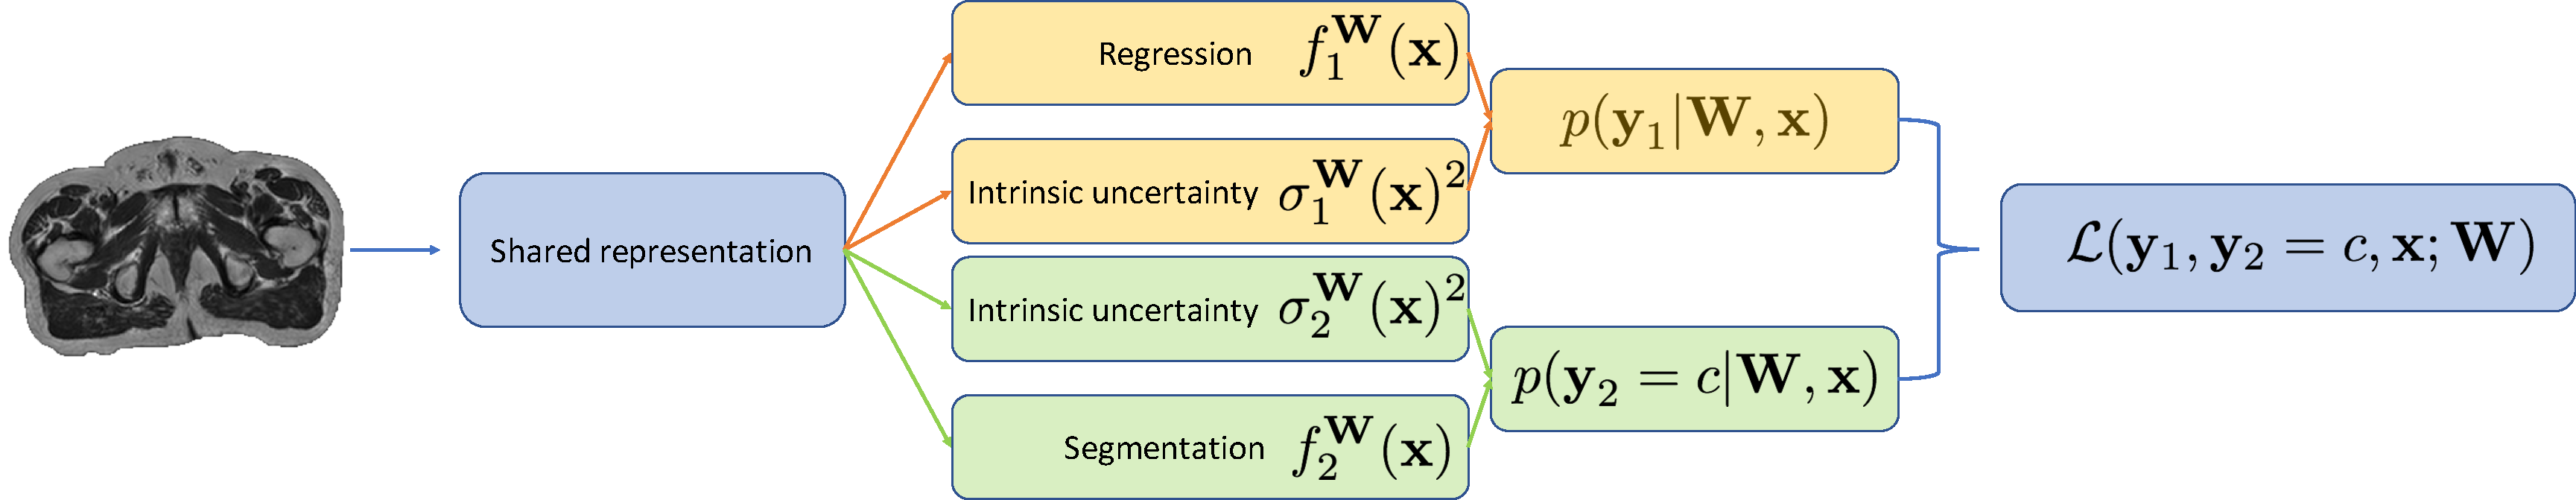
\includegraphics[height=0.185\textwidth]{chapter_5/figures/final_for_ryu_MT.pdf}
		\caption{Multi-task learning architecture. The predictive mean and variance $[f^{\mathbf{W}}_i(\text{\textbf{x}}), \sigma_{i}^{\mathbf{W}}(\text{\textbf{x}})^{2}]$ are estimated for the regression and segmentation. The task-specific likelihoods p$\left(\text{\textbf{y}}_{i}|\text{\textbf{W}},\text{\textbf{x}}\right)$ are combined to yield the multi-task likelihood p$\left(\text{\textbf{y}}_{1}, \text{\textbf{y}}_{2}|\text{\textbf{W}},\mathbf{x}\right)$.} 
		\label{fig:diagram}
	\end{figure}
    
The rationale behind shared layers is to learn a joint representation between two tasks to regularise the learning of features for one task by using cues from the other. We used a high-resolution network architecture (HighResNet) \cite{li2017compactness} as the shared trunk of the model for its compactness and accuracy shown in brain parcellation. HighResNet is a fully convolutional architecture that utilises dilated convolutions and residual connections to produce an end-to-end mapping from an input patch (\textbf{x}) to voxel-wise predictions (\textbf{y}).  
%The network is capable of representing the data at multiple scales  \todo[color=red!40]{(Ryu): Not sure if this statement is correct. The original dilated conv paper used a context aggregation module which applies 3x3 dilated conv kernels of different dilation factors to the same input features. This allows for multi-scale representation. But, in HighResNet, each dilated conv layer has a fixed dilation factor, right? I agree that this increases the receptive efficiently without pooling.} by increasing the dilation factor of the convolutions at each successive layer. The residual blocks facilitate the modeling of an identity mapping in feature space. Each residual block combines a convolutional layer, an activation layer and a batch-normalisation layer.   

%\subsubsection{Task-specific networks}
% (Ryu) in progress: The final layer of the representation network is split into two task-specific compartments (Fig. \ref{fig:diagram}). Each compartment consists of two networks which operate on the output of representation network and defines the likelihood function $p\left(\text{\textbf{y}}_{i}|f^{\text{\textbf{W}}}(\text{\textbf{x}})\right)$ for each task $i=1, 2$. 

% The goal of each branch is to predict the output of the regression ($y_{1}$), the uncertainty in the regression ($\sigma_{1}$) in addition to the prediction and uncertainty of the segmentation ($y_{2}$ and $\sigma_{2}$). We applied successive convolutional layers with associated activation and batch-normalisation layers to learn task-specific features. Given the predictions, we formulate the likelihood $p\left(\text{\textbf{y}}_{i}|f^{\text{\textbf{W}}}(\text{\textbf{x}})\right)$ for each task $i=1, 2$ given the task-specific estimates and the parameters \textbf{W} for the multi-task network. A joint-likelihood for the network is formulated by considering $p\left(\text{\textbf{y}}_{1},\text{\textbf{y}}_{2}|f^{\text{\textbf{W}}}(\text{\textbf{x}})\right)$ = $\prod_{i} p\left(\text{\textbf{y}}_{i}|f^{\text{\textbf{W}}}(\text{\textbf{x}})\right)$. The methodology for formulating $p\left(\text{\textbf{y}}_{1},\text{\textbf{y}}_{2}|f^{\text{\textbf{W}}}(\text{\textbf{x}})\right)$ with \emph{heteroscedastic} and \emph{parameter} uncertainty is described in the following sections. \todo[color=red!40]{(Ryu) Remove f - just need $p(y|x, W)$. I think the factorisation of lkhd over tasks directly comes from the architecture directly. Will reflect this thought later.}

The final layer of the shared representation is split into two task-specific compartments (Fig. \ref{fig:diagram}). Each compartment consists of two fully convolutional networks which operate on the output of representation network and together learn task-specific representation and define likelihood function $p\left(\text{\textbf{y}}_{i}|\text{\textbf{W}},\textbf{x}\right)$ for each task $i=1, 2$ where \text{\textbf{W}} denotes the set of all parameters of the model. 
%deleted{FELIX] At test time, we use the expectation of these likelihoods as the final estimates for CT intensity value and segmentation label. 
% The final layer of the representation network is split into four individual branches \textcolor{green}{each targeting a specific task: prediction of the regression (resp. segmentation) output $y_{1}$ (resp. $y_{2}$) and of their associated uncertainty $\sigma_1$ (resp. $\sigma_2$)}
% versino 1for each task (Fig. \ref{fig:diagram}). The goal of each branch is to predict the output of the regression ($y_{1}$), the uncertainty in the regression ($\sigma_{1}$) in addition to the prediction and uncertainty of the segmentation ($y_{2}$ and $\sigma_{2}$). Given the predictions, we formulate the likelihood $p\left(\text{\textbf{y}}_{i}|f^{\text{\textbf{W}}}(\text{\textbf{x}})\right)$ for each task $i=1, 2$ given the task-specific estimates and the parameters \textbf{W} for the multi-task network. A joint-likelihood for the network is formulated by considering $p\left(\text{\textbf{y}}_{1},\text{\textbf{y}}_{2}|f^{\text{\textbf{W}}}(\text{\textbf{x}})\right)$ = $\prod_{i} p\left(\text{\textbf{y}}_{i}|f^{\text{\textbf{W}}}(\text{\textbf{x}})\right)$. The methodology for formulating $p\left(\text{\textbf{y}}_{1},\text{\textbf{y}}_{2}|f^{\text{\textbf{W}}}(\text{\textbf{x}})\right)$ with \emph{heteroscedastic} and \emph{parameter} uncertainty is described in the following sections. \todo[color=red!40]{(Ryu) Remove f - just need $p(y|x, W)$. I think the factorisation of lkhd over tasks directly comes from the architecture directly. Will reflect this thought later.}

%A successful probabilistic radiotherapy planning requires both the high quality OAR segmentation, and the Hounsfield Unit prediction along with its associated uncertainty. %\textcolor{green}{some motivation for modelling uncertainty.}
%to better simulate the expected dose delivery . 
\subsection{Task weighting with heteroscedastic uncertainty.}
Previous probabilistic multitask learning methods based on deep learning \cite{kendall2017multi} assumed constant intrinsic uncertainty in respective tasks. In our context, this means that the inherent ambiguity present in synthesis or segmentation tasks do not depend on the spatial locations within an image volume. This is a highly unrealistic assumption as these tasks can be more challenging on some anatomical structures (e.g. tissue boundaries) than others. In order to capture potential spatial variation in intrinsic uncertainty, we adapt the \emph{heteroscedastic} (data-dependent) noise model to our multitask learning problem.   

In particular, for the CT synthesis task, we define our likelihood as a normal distribution $p\left(\text{\textbf{y}}_{1}|\mathbf{W},\mathbf{x}\right) = \mathcal{N}(f^{\text{\textbf{W}}}_1(\text{\textbf{x}}), \sigma_{1}^{\text{\textbf{W}}}(\text{\textbf{x}})^{2})$
where mean $f^{\text{\textbf{W}}}_1(\text{\textbf{x}})$ and variance $\sigma_{1}^{\text{\textbf{W}}}(\text{\textbf{x}})^{2}$ are modelled by the regression output and uncertainty branch as functions of the input patch $\mathbf{x}$ (see Fig.\ref{fig:diagram}). We define the task loss for CT synthesis to be the negative log-likelihood $\mathcal{L}_{1}(\text{\textbf{y}}_{1},\mathbf{x};\mathbf{W})= \frac{1}{2\sigma_{1}^{\text{\textbf{W}}}(\text{\textbf{x}})^{2}}||\text{\textbf{y}}_{1}-f^{\text{\textbf{W}}}_1(\text{\textbf{x}})||^{2} + \text{log}\sigma_{1}^{\text{\textbf{W}}}(\text{\textbf{x}})^{2}$. This loss encourages assigning high-uncertainty to regions of high errors, enhancing the robustness of the network against noisy labels and outliers, which are prevalent at organ boundaries especially close to the bone.
%This objective acts as a learned loss attenuation since the network can learn to attenuate the effect of erroneous predictions by predicting higher uncertainty in these regions. This is of particular importance when regressing voxel intensities at organ boundaries especially close the bone, which are prone to errors.
% (version 2) We introduce the \emph{heteroscedastic} noise model to approximate the variation in intrinsic uncertainty across the image. In contrast to \emph{homoscedatic} uncertainty ($\sigma_{i}$) which is assumed constant across the image, \emph{heteroscedasticity} is data-dependent ($\bm{\sigma}_{i}(\text{\textbf{x}})$). For the CT synthesis task, we define our likelihood as a normal distribution with mean given by the regression output $p\left(\text{\textbf{y}}_{1}|\mathbf{W},\mathbf{x}\right) = \mathcal{N}(f^{\text{\textbf{W}}}_1(\text{\textbf{x}}), \sigma_{1}^{\text{\textbf{W}}}(\text{\textbf{x}})^{2})$. The negative log-likelihood is given by $-\text{log}\,p\left(\text{\textbf{y}}_{1}|\mathbf{W},\mathbf{x}\right) = \frac{1}{2\sigma_{1}^{\text{\textbf{W}}}(\text{\textbf{x}})}||\text{\textbf{y}}_{1}-f_{1}(\text{\textbf{x}})^{\text{\textbf{W}}}||^{2} + \text{log}\sigma_{1}^{\text{\textbf{W}}}(\text{\textbf{x}})^{2}$. This likelihood acts as a learned loss attenuation since the network can learn to attenuate the effect of erroneous predictions by predicting higher uncertainty in these regions. This is of particular importance when regressing voxel intensities at organ boundaries especially close the bone, which are prone to errors.

For the segmentation, we define the classification likelihood as softmax function of scaled logits i.e. $p\left(\text{\textbf{y}}_{2}|\textbf{W},\mathbf{x}\right) = \text{Softmax}\big{(}f_{2}^{\text{\textbf{W}}}(\text{\textbf{x}})/2\sigma^{\mathbf{W}}_{2}(\text{\textbf{x}})^2\big{)}$ where the segmentation output $f_{2}^{\text{\textbf{W}}}(\text{\textbf{x}})$ is scaled by the uncertainty term $\sigma^{\mathbf{W}}_{2}(\text{\textbf{x}})^2$ before softmax (Fig.\ref{fig:diagram}). As the uncertainty term $\sigma^{\mathbf{W}}_{2}(\text{\textbf{x}})$ increases, the Softmax output approaches a uniform distribution, which corresponds to the maximum entropy discrete distribution. We simplify the scaled Softmax likelihood by considering an approximation in \cite{kendall2017multi} 
$$\frac{1}{\sigma^{2}}\sum_{c'}\text{exp}(\frac{1}{2\sigma^{\mathbf{W}}_{2}(\text{\textbf{x}})^2}f^{\text{\textbf{W}}}_{2,c'}(\text{\textbf{x}})) \approx \left(\sum_{c'}\text{exp}(f^{\mathbf{W}}_{2,c'}(\text{\textbf{x}}))\right)^{1/2\sigma^{\mathbf{W}}_{2}(\text{\textbf{x}})^2}$$ where $c'$ is denotes a segmentation class. This yields the NLL task-loss of the form $\mathcal{L}_{2}(\text{\textbf{y}}_{2}=c,\mathbf{x};\mathbf{W}) \approx \frac{1}{2\sigma^{\mathbf{W}}_{2}(\text{\textbf{x}})^2} \text{CE}(f_{2}^{\text{\textbf{W}}}(\text{\textbf{x}}),\text{\textbf{y}}_{2}=c)+ \text{log}\sigma^{\mathbf{W}}_{2}(\text{\textbf{x}})^2$, where CE denotes cross-entropy.
%(f^{\textbf{W}},\textbf{y}}_{2}) + \text{log}\sigma_{2}^{2}(\text{\textbf{x}})
%$\bm{\mathcal{L}}_{2}(\text{\textbf{y}}_{2},\mathbf{x};\mathbf{W}) \approx -\frac{1}{2\sigma^{2}_{2}(\text{\textbf{x}})} \text{log}\left(\text{softmax}(f^{\text{\textbf{W}}}(\text{\textbf{x}}))\right) + \text{log}\sigma_{2}^{2}(\text{\textbf{x}})$. Consequently, the multi-task loss with heteroscedastic weighting that is minimised is:
Finally, assuming that the two tasks $\text{\textbf{y}}_{1},\text{\textbf{y}}_{2}$ are statistically independent given the input image $\mathbf{x}$,  the joint likelihood factorises over tasks  $p\left(\text{\textbf{y}}_{1},\text{\textbf{y}}_{2}|\mathbf{W},\mathbf{x}\right)=p\left(\text{\textbf{y}}_{1}|\mathbf{W},\mathbf{x}\right)p\left(\text{\textbf{y}}_{2}|\mathbf{W},\mathbf{x}\right)$, and thus we can derive the NLL loss for the dual-task model as
\begin{equation*}
\mathcal{L}(\textbf{y}_{1},\textbf{y}_{2}=c,\mathbf{x};\mathbf{W}) =\frac{||\text{\textbf{y}}_{1}-f^{\text{\textbf{W}}}_1(\text{\textbf{x}})||^{2}}{2\sigma_{1}^{\text{\textbf{W}}}(\text{\textbf{x}})^{2}} + \frac{\text{CE}(f_{2}^{\text{\textbf{W}}}(\text{\textbf{x}}),\text{\textbf{y}}_{2}=c)}{2\sigma^{\mathbf{W}}_{2}(\text{\textbf{x}})^2} + \text{log}\Big{(}\sigma^{\mathbf{W}}_{1}(\text{\textbf{x}})^2\sigma^{\mathbf{W}}_{2}(\text{\textbf{x}})^2\Big{)}\;
\end{equation*}
% \begin{equation}
% \mathcal{L}(\textbf{y}_{1},\textbf{y}_{2}=c,\mathbf{x};\mathbf{W}) = \sum_{i} \frac{1}{\sigma^{\mathbf{W}}_{i}(\text{\textbf{x}})^2}(\textbf{y}_{i},\mathbf{x};\mathbf{W}) + \text{log}\sigma^{\mathbf{W}}_{i}(\text{\textbf{x}})^2 \;
% \end{equation}
where the MSE and CE terms are weighted by the inverse of heteroscedastic intrinsic uncertainty terms $\sigma^{\mathbf{W}}_{i}(\text{\textbf{x}})^2$, that enables automatic weighting of task losses on a per-sample basis. The log-term controls the spread. 

\subsection{Parameter uncertainty with approximate Bayesian inference.} In data-scarce situations, the choice of best parameters is ambiguous, and resorting to a single estimate without regularisation often leads to overfitting. Gal et al.\cite{gal2016dropout} have shown that dropout improves the generalisation of a NN by accounting for \textit{parameter} uncertainty through an approximation of the posterior distribution over its weights $q(\mathbf{W}) \approx (\mathbf{W}|\mathbf{X},\mathbf{Y_1},\mathbf{Y_2})$ where $\mathbf{X} = \{\mathbf{x}^{(1)}, ..., \mathbf{x}^{(N)}\}$, $\mathbf{Y}_1 = \{\mathbf{y}_1^{(1)}, ..., \mathbf{y}_1^{(N)}\}$, $\mathbf{Y}_2	 = \{\mathbf{y}_2^{(1)}, ..., \mathbf{y}_2^{(N)}\}$ denote the training data. In this work, we also use dropout in our model to assess the benefit of modelling parameter uncertainty in the context of our multitask learning problem.

During training, for each input (or minibatch), network weights are drawn from the approximate posterior $w' \sim q(\textbf{\text{W}})$ to obtain the multi-task output (predictive mean and predictive variance), $\textbf{f}^{w'}(\text{\textbf{x}}):=[f^{w'}_1(\text{\textbf{x}}),f^{w'}_2(\text{\textbf{x}}), \sigma_{1}^{w'}(\text{\textbf{x}})^{2},\sigma_{2}^{w'}(\text{\textbf{x}})^{2}]$. At test time, for each input patch $\textbf{\text{x}}$ in a MR scan, we collect output samples $\{\textbf{f}^{\,w^{(t)}}(\text{\textbf{x}})\}_{t=1}^{\text{T}}$ by performing $T$ stochastic forward-passes with $\{w^{(t)}\}_{t=1}^{\text{T}}\sim q(\mathbf{W})$. For the regression, we calculate the expectation over the $T$ samples in addition to the variance, which is the \emph{parameter} uncertainty. For the segmentation, we compute the expectation of class probabilities to obtain the final labels. The \emph{parameter} uncertainty in the segmentation is obtained by considering variance of the stochastic class probabilities. The final predictive uncertainty is the sum of the \emph{intrinsic} and \emph{parameter} uncertainties.
%$[\hat{\textbf{\text{y}}}_{1},\hat{\textbf{\text{y}}}_{2},\bm{\hat{\sigma}}^{2}_{1},\bm{\hat{\sigma}}^{2}_{2}]=f^{\bm{\hat{\text{W}}}}(\text{\textbf{x}})$
% At test time, given an input patch in MR scan $\textbf{\text{x}}$, we estimate the predictive distribution $q(\hat{\textbf{\text{y}}}|\hat{\textbf{\text{x}}})$ by sampling from $q(\textbf{\text{W}})$ with $T$ stochastic-samples. For the regression, we calculate the expectation over the $T$ samples in addition to the variance, which is the \emph{parameter} uncertainty. For the segmentation, we perform consider the expectation of class probabilities to obtain the final labels. \emph{Parameter} uncertainty in the segmentation is obtained by considering variance of the stochastic class probabilities. The final predictive uncertainty is the sum of the \emph{intrinsic} and \emph{parameter} uncertainties. This reduces to the the \emph{parameter} uncertainty when no heteroscedastic noise is modelled. 
% During training, network weights are drawn from the approximate posterior $\hat{\text{W}} \sim q(\textbf{\text{W}})$ to obtain the multi-task output with predictive mean and predictive variance $[\hat{\textbf{\text{y}}}_{1},\hat{\textbf{\text{y}}}_{2},\bm{\hat{\sigma}}^{2}_{1},\bm{\hat{\sigma}}^{2}_{2}]=f^{\bm{\hat{\text{W}}}}(\text{\textbf{x}})$. 

% At test time, given an input patch in MR scan $\textbf{\text{x}}$, we estimate the predictive distribution $q(\hat{\textbf{\text{y}}}|\hat{\textbf{\text{x}}})$ by sampling from $q(\textbf{\text{W}})$ with $T$ stochastic-samples. For the regression, we calculate the expectation over the $T$ samples in addition to the variance, which is the \emph{parameter} uncertainty. For the segmentation, we perform consider the expectation of class probabilities to obtain the final labels. \emph{Parameter} uncertainty in the segmentation is obtained by considering variance of the stochastic class probabilities. The final predictive uncertainty in the multi-task network the sum of the \emph{intrinsic} and \emph{parameter} uncertainties. When no heteroscedastic noise is modelled, this uncertainty reduces to the \emph{parameter} uncertainty.

\subsection{Implementation details}\label{sec:imp_details} 
We trained our model on randomly selected 2D axial slices and reconstructed the 3D volume at test time. The representation network was composed of a convolutional layer followed by $3$ sets of twice repeated dilated convolutions with dilation factors $[1,2,4]$ and a final convolutional layer. Each layer ($l$) used a $3 \times 3$ kernel with features $f_{R}=[64, 64, 128, 256, 2048]$. Each task-specific branch was a set of $5$ convolutional layers of size $[256_{l=1, 2, 3, 4},n_{i,l=5}]$ where $n_{i,l=5}$ is equal to $1$ for regression and $\bm{\sigma}$ and equal to the number of segmentation classes. The first two layers were $3 \times 3$ kernels whilst the final convolutional layers were fully connected. A Bernouilli drop-out mask with probability $p=0.5$ was applied on the final layer of the representation network. We minimised the loss using ADAM with a learning rate $10^{-3}$ and trained for $19,000$ iterations. For the stochastic sampling, we performed model inference $10$ times at iterations $18000$ and $19000$ leading to a set of $T=20$ samples. 

\section{Experiments and Results}

%\subsubsection{Moved from section 2.3 Implementation details}
%\textcolor{green}{also considered a baseline model to perform single-task regression and segmentation. This was performed with and without drop-out. This baseline was composed of only the representation network with $\nicefrac{1}{2}f_{R}$ and an extra fully-connected layer to output $\text{\textbf{y}}$.}
%\todo[color=green!40]{Integrate the above paragraph into one of the subsections in section 3}

\subsection{Data}
We validated on $15$ prostate cancer patients, who each had a T2-weighted MR image (3T, $1.46\times1.46\times5$mm$^{3}$) and a CT image (140kVp, $0.98\times0.98\times1.5$mm$^{3}$) acquired on the day. Organ delineation was performed by a clinician with labels for the left and right femur head, bone, prostate, rectum and bladder. All images were resampled to isotropic resolution. The CT scans were spatially aligned with the T2 scans using the method of Burgos et al. \cite{ninon2017}. In the segmentation, we predicted labels for the background, left/right femur head, prostate, rectum and bladder. The bone region was used for quantifying the synCT.

\subsection{Experiments}
We performed a 3-fold cross-validation. Statistics over all hold-out sets are reported. We considered four separate models; 1) baseline networks for regression/segmentation (M1), 2) baseline network with drop-out for regression/segmentation (M2a), 3) the baseline with drop-out and heteroscedastic noise (M2b), 4) multi-task network using homoscedastic task weighting (M3) \cite{kendall2017multi} and 5) multi-task network using task-specific heteroscedastic noise and drop-out (M4). The baseline networks used only the representation network with $\nicefrac{1}{2}f_{R}$ and a fully-connected layer for the final output. We also compared our results against the current state of the art in atlas propagation (AP) \cite{ninon2017}, which was validated on the same dataset.

\subsection{Model performance}
\begin{table}[!b]
\caption{Model comparison. Bold values indicate where a model was significantly worse than M4 $p<0.05$. No data was available for significance testing with AP. M2b was statistically better $p<0.05$ than M4 in the prostate segmentation.}
\begin{center}
\scalebox{0.90}{
\begin{tabular}{lccccccc}
\toprule
        Models & All & Bone & $L$ femur & $R$ femur & Prostate & Rectum & Bladder \\
\midrule
\multicolumn{8}{c}{Regression - synCT - Mean Absolute Error (HU)} \\
\midrule
M1 			   & \textbf{48.1(4.2)} & \textbf{131(14.0)}  & 78.6(19.2) & \textbf{80.1(19.6)}   & \textbf{37.1(10.4)}  & 63.3(47.3)  & \textbf{24.3(5.2)} \\
M2a 			   & \textbf{47.4(3.0)} & \textbf{130(12.1)}  & 78.0(14.8) & 77.0(13.0)   & \textbf{36.5(7.8)}  & 67(44.6)  & \textbf{24.1(7.5)} \\
M2b \cite{kendall2017uncertainties} & 44.5(3.6) & 128(17.1)  & 75.8(20.1) & 74.2(17.4)   & 31.2(7.0)  & 56.1(45.5)  & 17.8(4.7) \\
M3 \cite{kendall2017multi}& 44.3(3.1) & 126(14.4)  & 74.0(19.5) & 73.7(17.1)   & 29.4(4.7)  & 58.4(48.0) & 18.2(3.5) \\
AP \cite{ninon2017}& 45.7(4.6) & 125(10.3) & - & - & - & - & - \\
M4 (ours) 			   & 43.3(2.9) & 121(12.6)  & 69.7(13.7) & 67.8(13.2)   &28.9(2.9)  & 55.1(48.1) & 18.3(6.1) \\
\midrule
\multicolumn{8}{c}{Segmentation - OAR - Fuzzy DICE score} \\
\midrule
M1 & - & - & 0.91(0.02) & 0.90(0.04) & 0.67(0.12) & 0.70(0.15) & 0.92(0.05) \\
M2a & - & - & 0.85(0.03) & 0.90(0.04) & 0.66(0.12) & 0.69(0.13) & 0.90(0.07) \\
M2b \cite{kendall2017uncertainties} & - & - & 0.92(0.02) & 0.92(0.01) & 0.77(0.07) & 0.74(0.13) & 0.92(0.03) \\
M3 \cite{kendall2017multi}& - & - & 0.92(0.02) & 0.92(0.02) & 0.73(0.07) & 0.76(0.10) & 0.93(0.02) \\
AP \cite{ninon2017} & - & - & 0.89(0.02) & 0.90(0.01) & 0.73(0.06) & 0.77(0.06) & 0.90(0.03) \\
M4 (ours) & - & - & 0.91(0.02) & 0.91(0.02) & 0.70(0.06) & 0.74(0.12) & 0.93(0.04) \\
\bottomrule
\end{tabular}}
\end{center}
\label{tab:table}
\vspace{-10mm}
\end{table}
We calculated the Mean Absolute Error (MAE) between the predicted and reference scans across the body and at each organ (Tab. \ref{tab:table}). The fuzzy DICE score between the probabilistic segmentation and the reference was calculated for the segmentation (Tab. \ref{tab:table}). Best performance was in our presented method (M4) for the regression across all segmentation masks except at the bladder. Application of the multi-task heteroscedastic network with drop-out (M4) produced the most consistent synCT across all models with the lowest average MAE and the lowest variation across patients ($43.3\pm2.9$ versus $45.7\pm4.6$ \cite{ninon2017} and $44.3\pm3.1$ \cite{kendall2017multi}). This was significant lower when compared to M1 ($p<0.001$) and M2 ($p<0.001$). This was also observed at the bone and prostate ($p<0.001$). Whilst differences at $p<0.05$ levels of significance was not observed versus M2b and M3, the consistent lower MAE and standard deviation across patients in M4 demonstrates the added benefit of modelling heteroscedastic noise and the inductive transfer from the segmentation task. Moreover, we performed better than the current state of the art in atlas propagation \cite{ninon2017}. despite equivalence with the state of the art (Tab. \ref{tab:table}), we did not observe any significant differences between our model and the baselines despite an improvement in mean DICE at the prostate and rectum ($0.70\pm0.06$ and $0.74\pm0.12$) versus the baseline M1 ($0.67\pm0.12$, $0.70\pm0.15$). The \emph{intrinsic uncertainty} (Fig. \ref{fig:diagram2}) models the uncertainty specific to the data and thus penalises regions of high error leading to an under-segmentation yet with higher confidence in the result.

\begin{figure}[!t]
		\centering
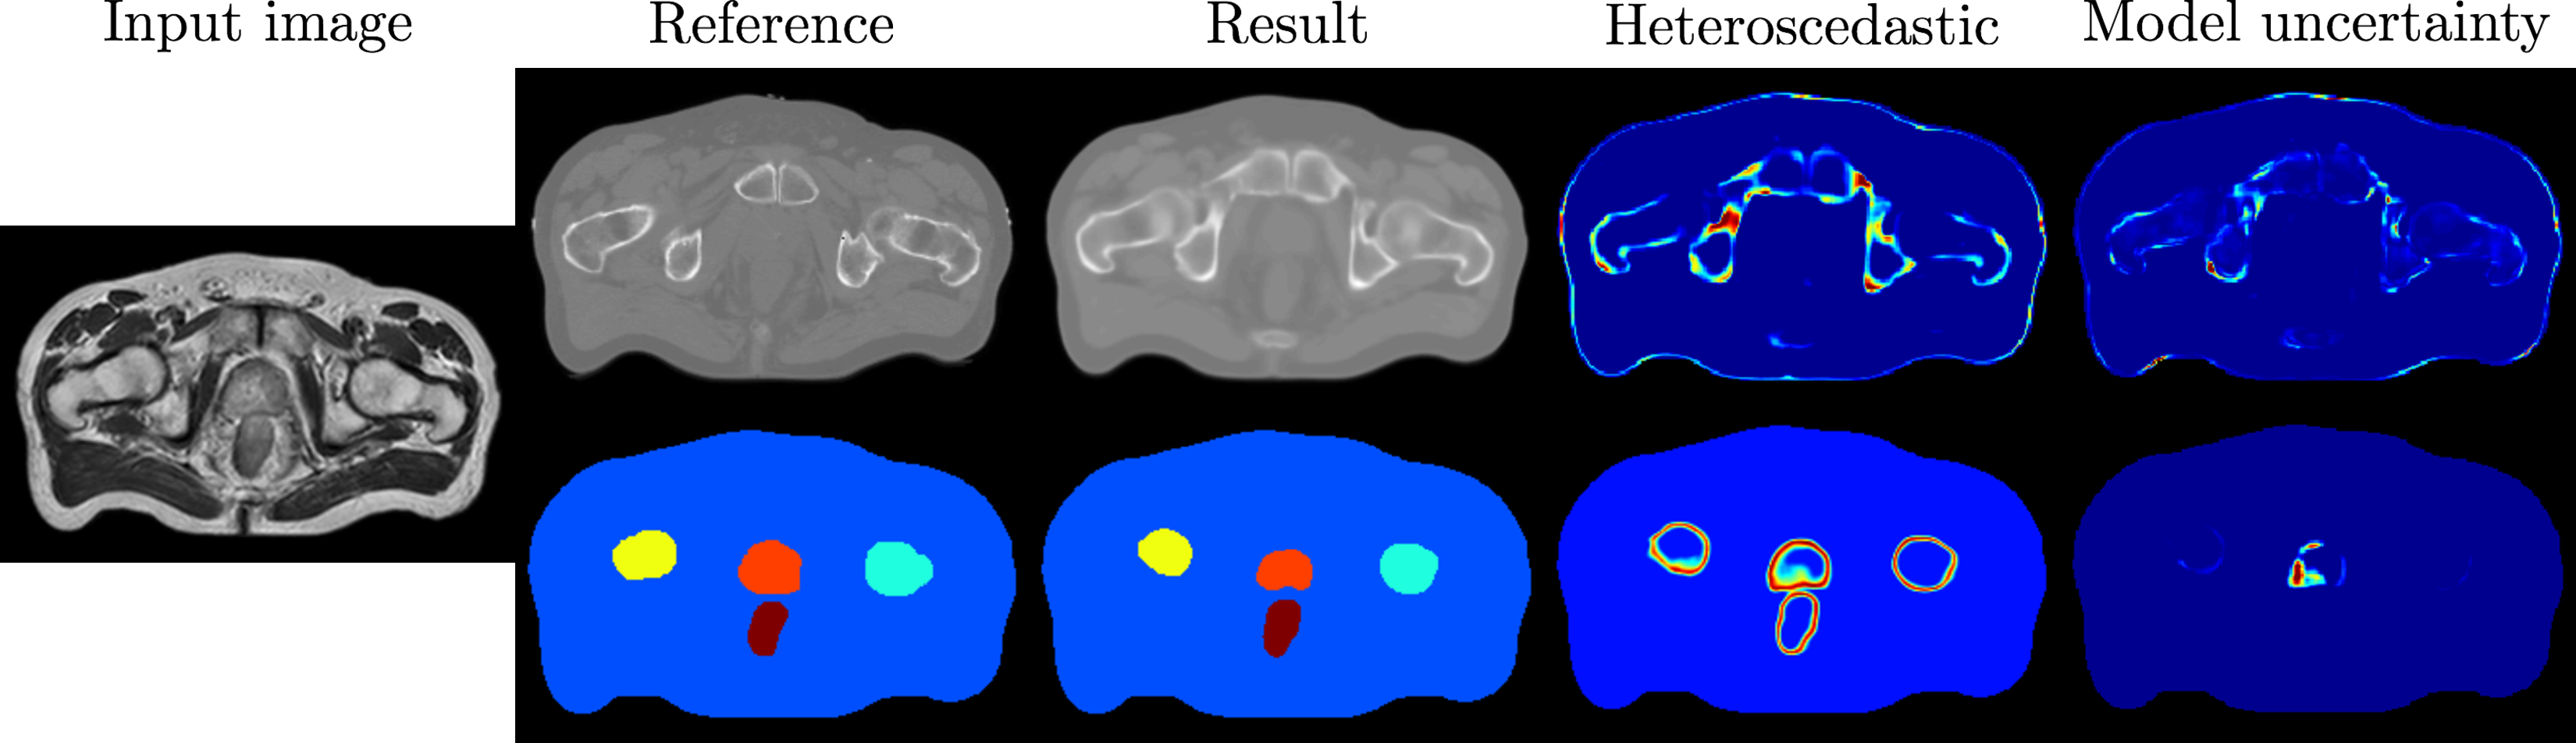
\includegraphics[height=0.275\textwidth]{chapter_5/figures/figure_1_res.pdf}
		\caption{Example output from the proposed network. The heteroscedastic intrinsic and the parameter uncertainty both correlate strongly with regions of high contrast (bone in the regression), organ boundary (segmentation) and errors in the output.} 

		\label{fig:diagram2}
        \vspace{-2mm}
\end{figure}

\subsection{Uncertainty estimation for radiotherapy}
We tested the ability of the multi-task heteroscedastic network to better predict associated uncertainties in the synCT error. To verify that our network produces clinically viable samples for treatment planning, we quantified the distribution of regression z-scores for the multi-task heteroscedastic and homoscedastic models. In the former, the total predictive uncertainty is the sum of the \emph{intrinsic} and \emph{parameter} uncertainties, which is used to normalise the error between the synCT and the reference. This should lead to a better approximation of the variance in the model. In contrast, the total uncertainty in the latter reduces to the variance of the stochastic test-time samples. This is likely to lead to a mis-calibrated variance. A $\chi^{2}$ goodness of fit test was performed, showing that the homoscedastic z-score distribution is not normally distributed ($0.82 \pm 0.54$, $p<0.01$) in contrast to the heteroscedastic model ($0.04 \pm 0.84$, $p>0.05$), which has overestimated the variance. This is apparent in Fig. \ref{fig:diag3} where there is greater confidence in the synCT produced by our model in contrast the homoscedastic case.

The predictive uncertainty can be exploited for quality assurance (Fig. \ref{fig:diagram4}). There may be issues whereupon time differences have caused variations in bladder and rectum filling across MR and CT scans causing patient variability in the training data. This is exemplified by large errors in the synCT at the rectum (Fig. \ref{fig:diagram4}) and quantified by large localised z-scores (Fig. \ref{fig:diagram4}g), which correlate strongly with the \emph{intrinsic} and \emph{parameter} uncertainty across tasks.

\begin{figure}[!t]
  \centering
	\begin{subfigure}[]{0.7\linewidth}
		\caption{Comparison of error quantification}	
		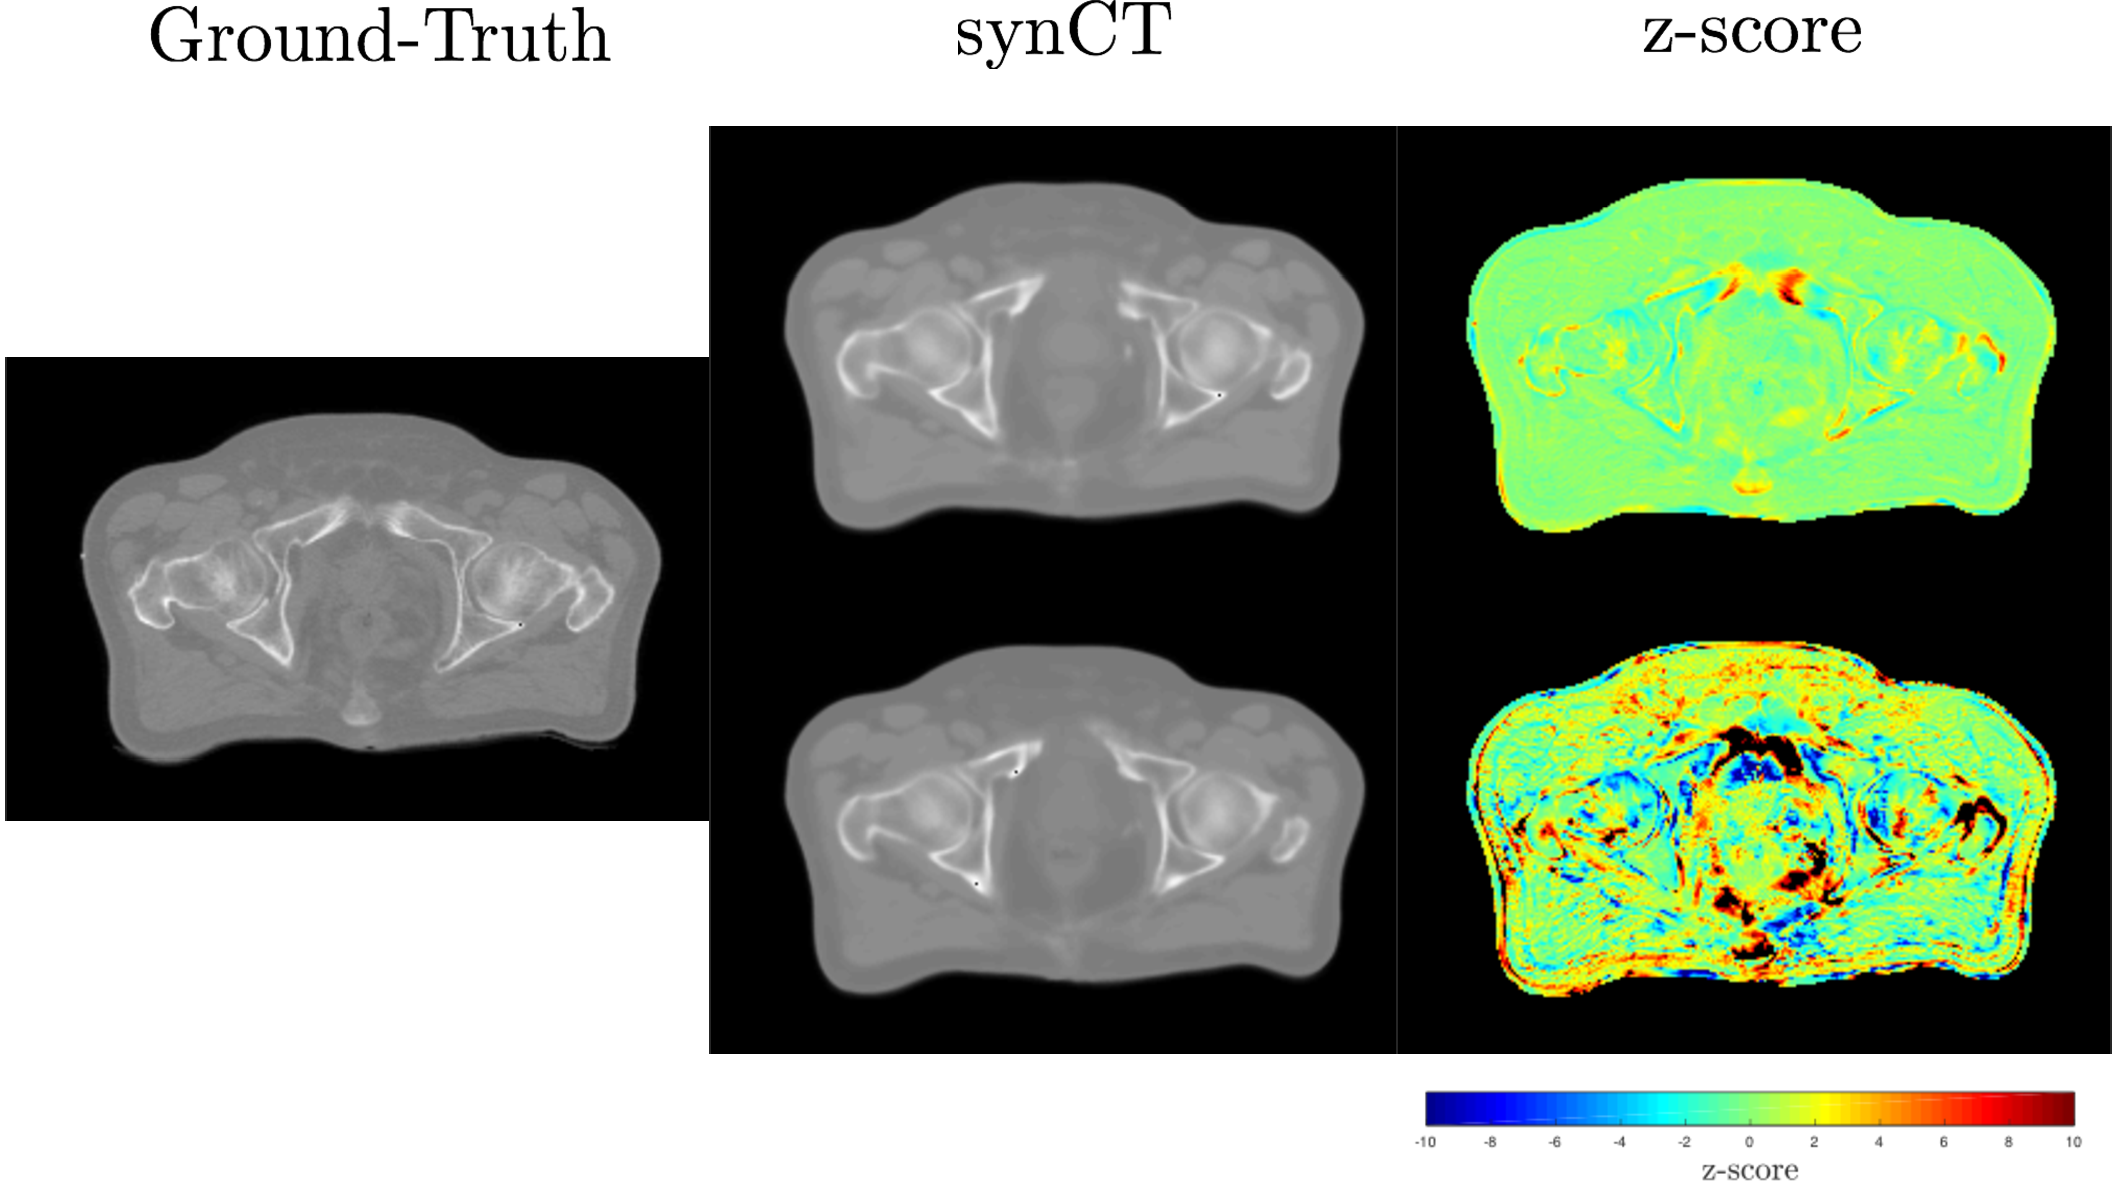
\includegraphics[width=\linewidth]{chapter_5/figures/fig_z_1.pdf}
	\end{subfigure}
	\begin{subfigure}[]{0.6\linewidth}
		\caption{z-score distribution}
		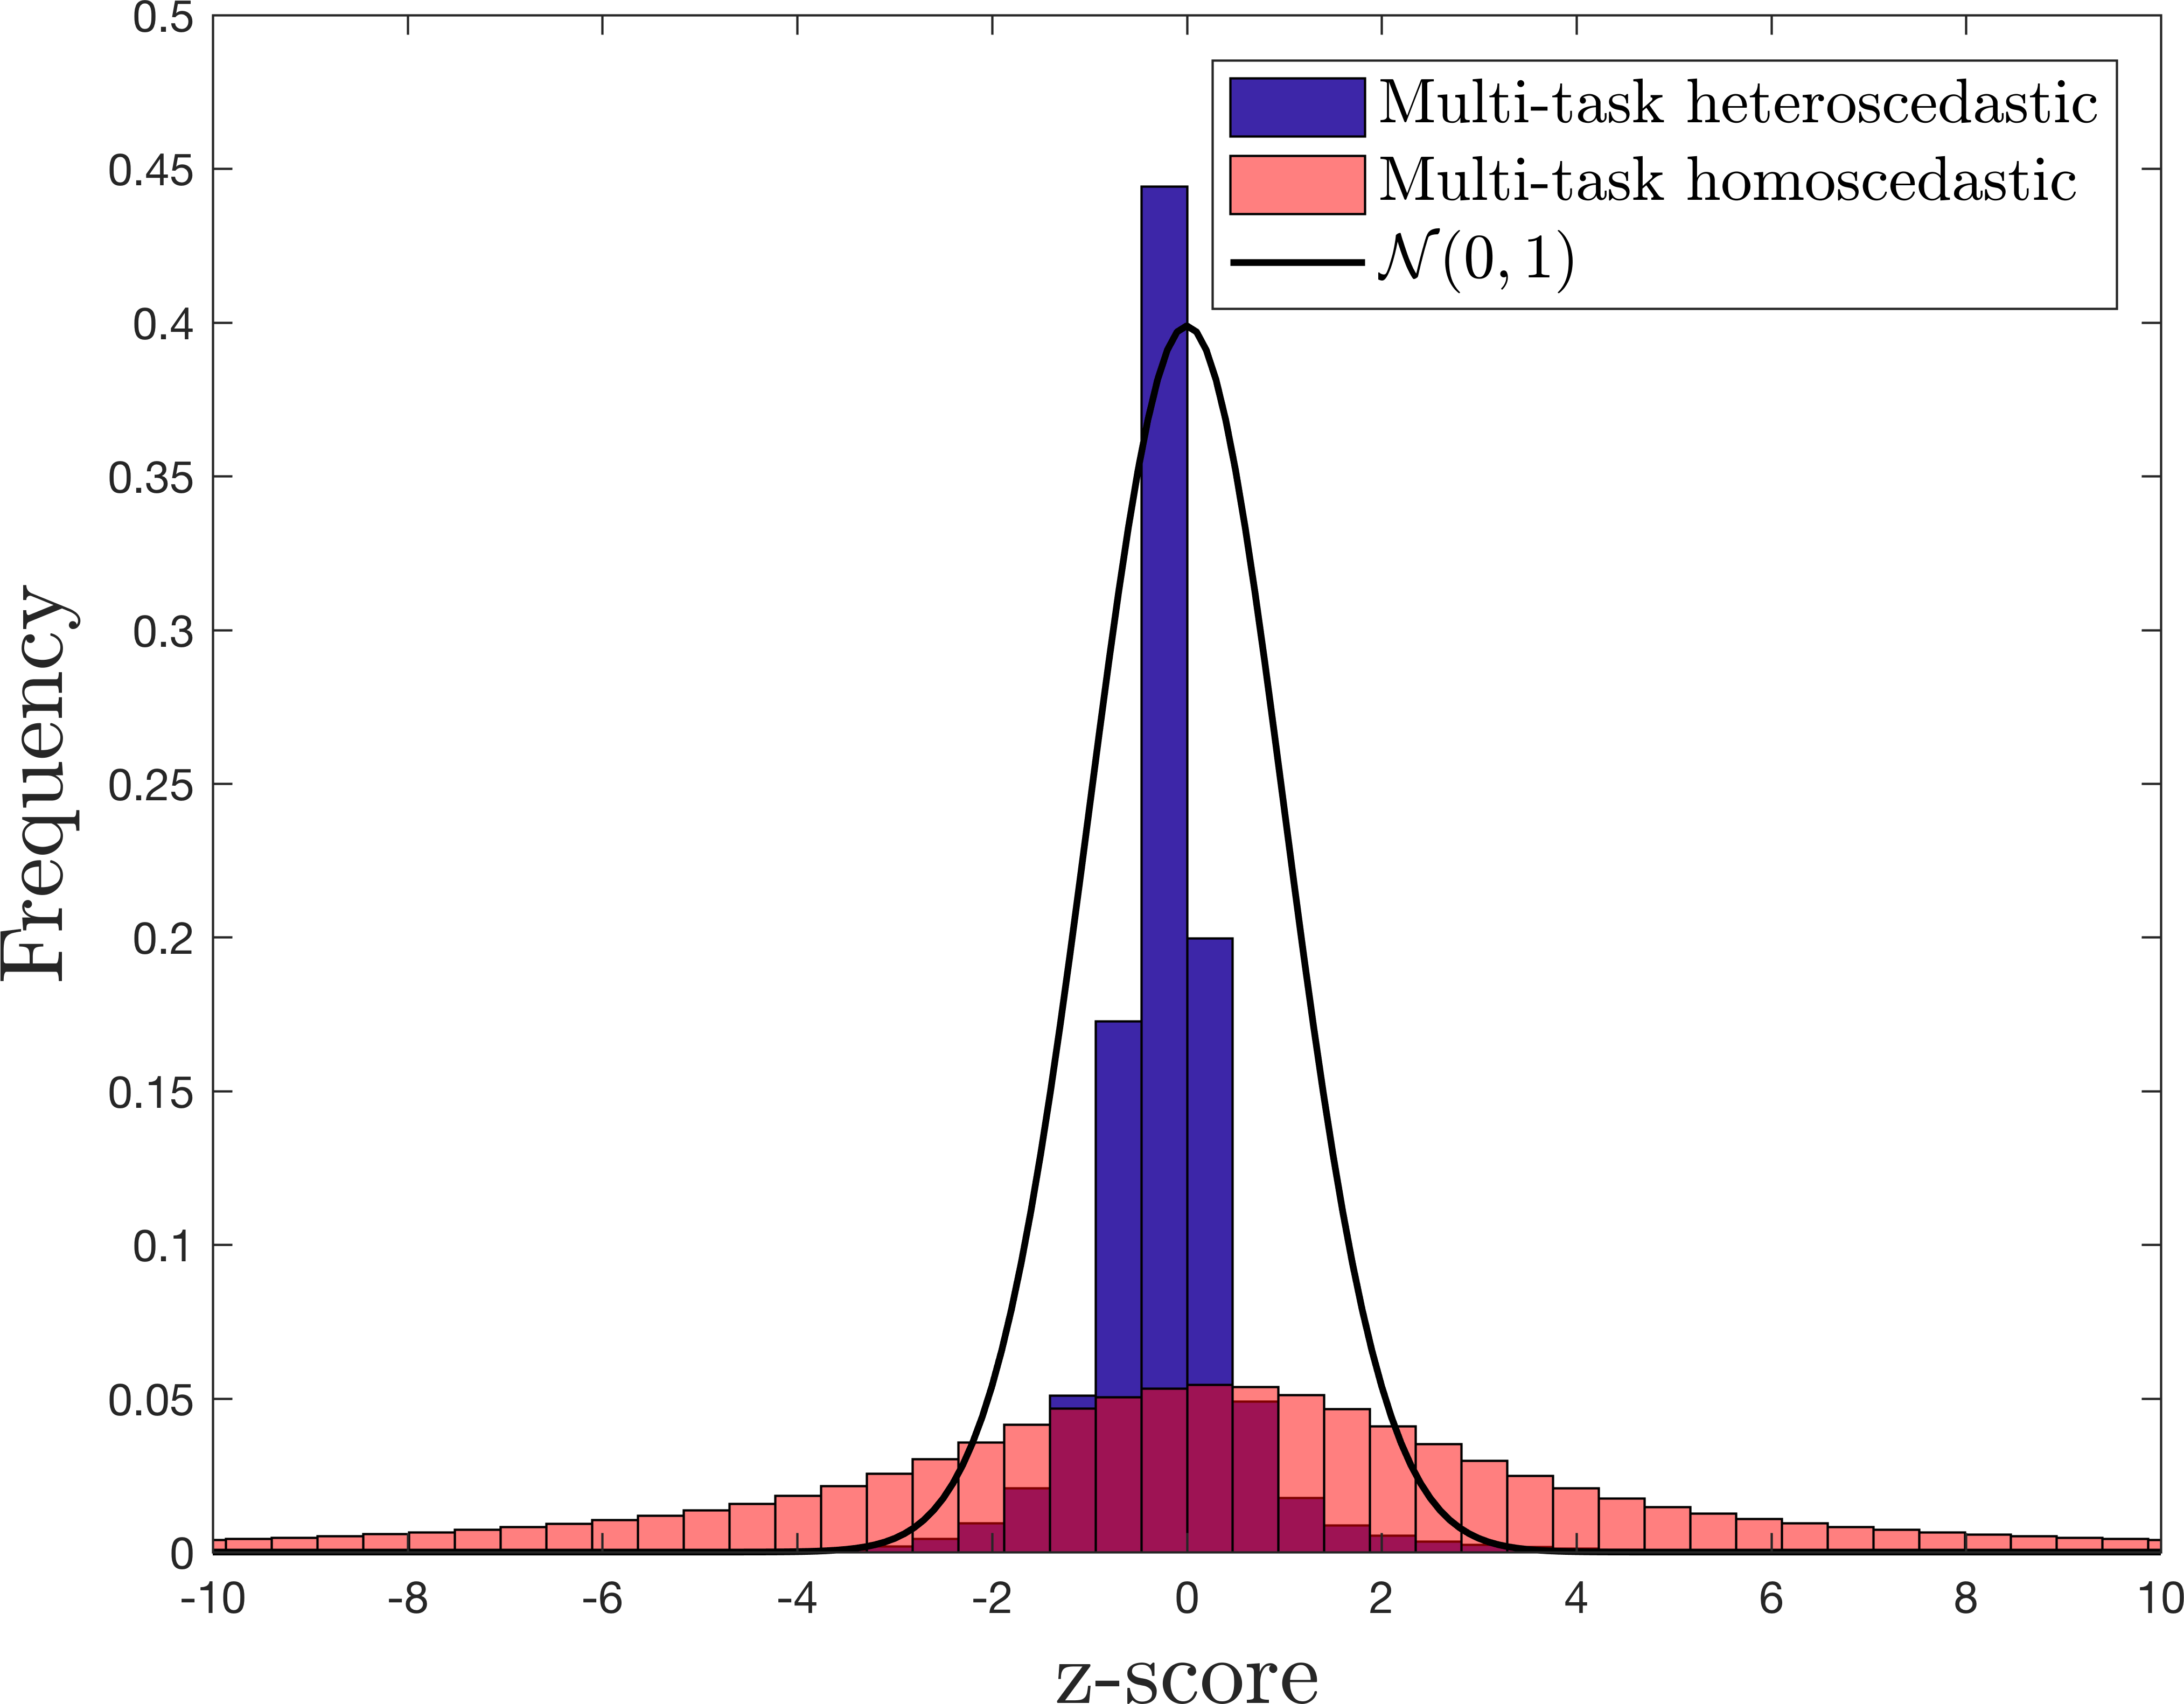
\includegraphics[width=\linewidth]{chapter_5/figures/fig_z_2.png}
	\end{subfigure}
	\caption{a) synCTs and z-scores for the same subject between M4 (top) and M3 (bottom) models. b) z-score distribution of all patients ($15$) between both models.}
	\label{fig:diag3}
\end{figure}

\begin{figure}[!t]
	\centering
	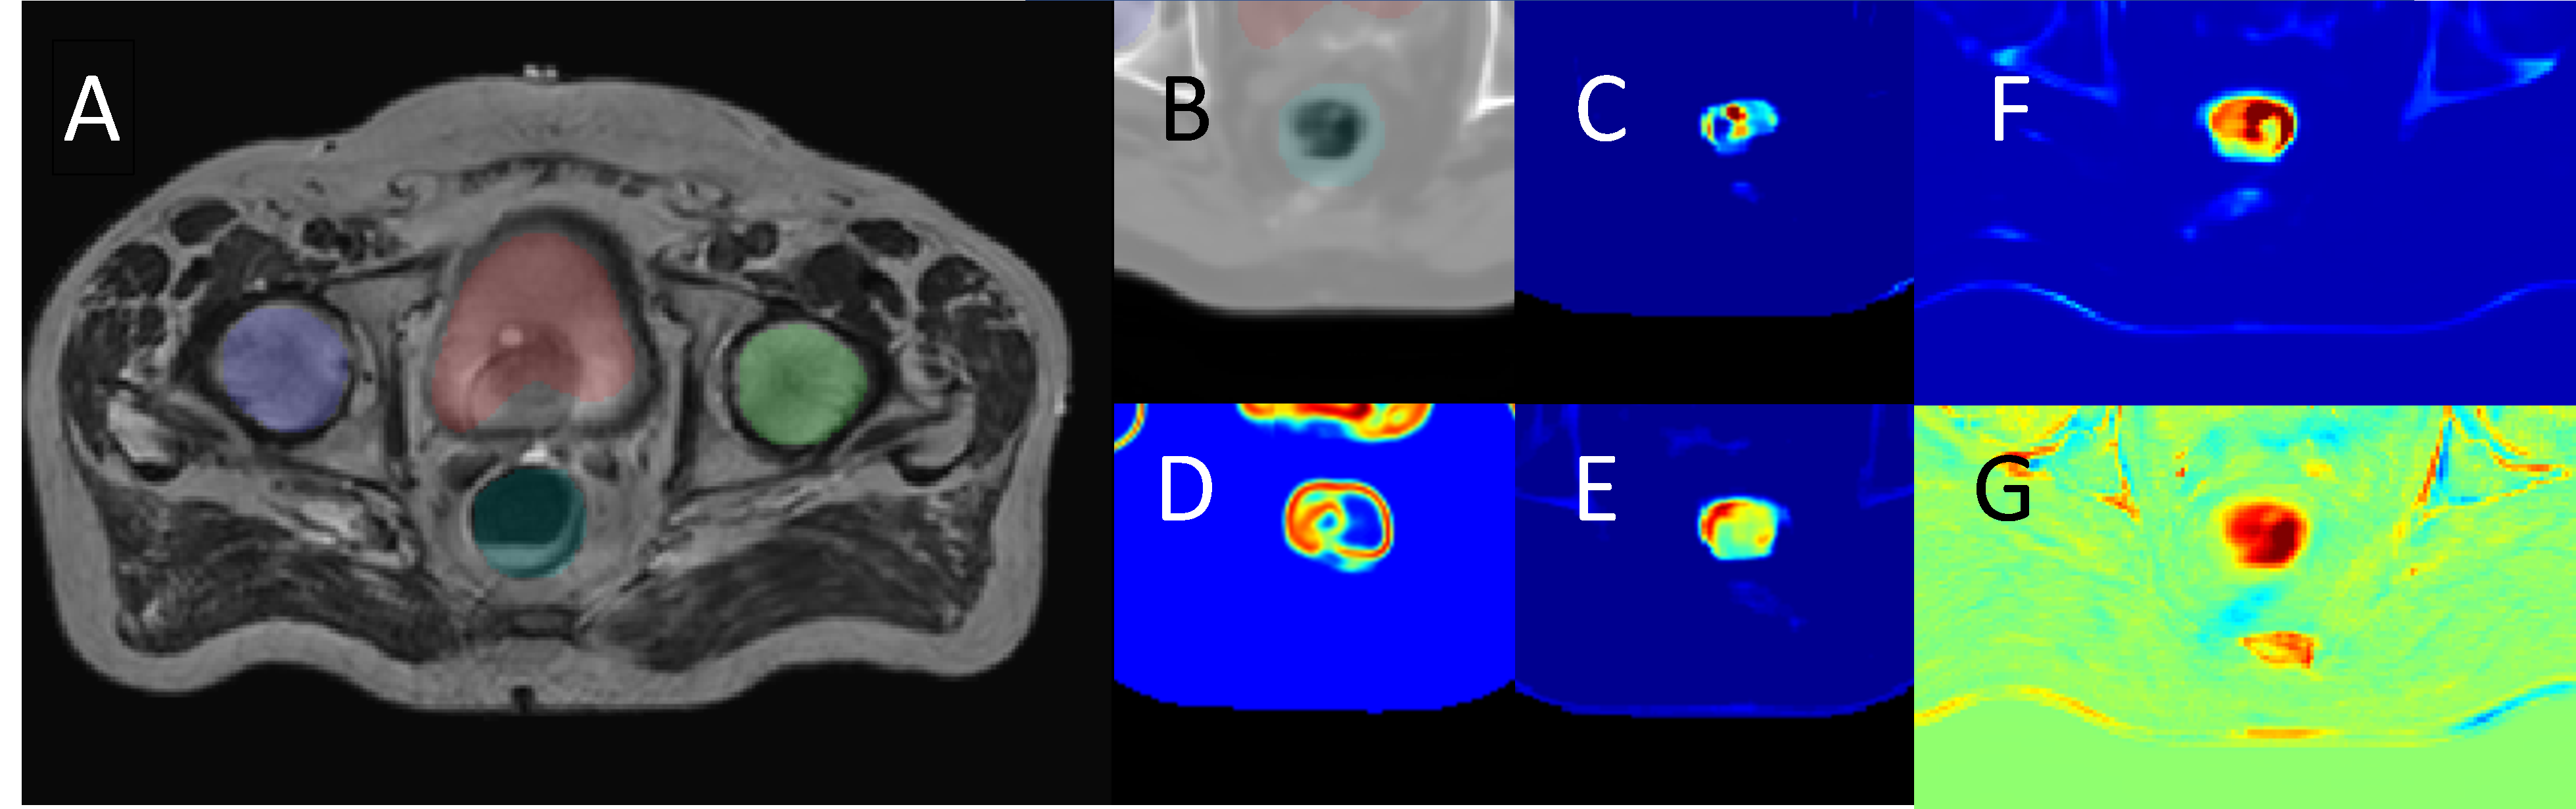
\includegraphics[width=\linewidth]{chapter_5/figures/figure_unc_2.pdf}
	\caption{Uncertainty in areas prone to errors. a) T2 with reference segmentation, b) synCT with errors at the rectum, c) parameter uncertainty in synCT, d) intrinsic uncertainty in the segmentation, e) intrinsic uncertainty in the regression, f) total predictive uncertainty in the regression and g) error in HU (range [-750HU, 750HU]).} 
	\label{fig:diagram4}
\end{figure}

\section{Conclusions}

We have proposed a probabilistic dual-network that combines uncertainty modelling with multi-task learning. Our network extends prior work in multi-task learning by integrating heteroscedastic uncertainty modelling to naturally weight task losses and maximize inductive transfer between tasks. We have demonstrated the applicability of our network in the context of MR-only radiotherapy treatment planning.  The model simultaneously provides the generation of synCTs, the segmentation of OARs and quantification of predictive uncertainty in both tasks. We have shown that a multi-task framework with heteroscedastic noise modelling leads to more accurate and consistent synCTs with a constraint on anatomical consistency with the segmentations. Importantly, we have demonstrated that the output of our network leads to consistent anatomically correct stochastic synCT samples that can potentially be effective in treatment planning. 





%delted: as they assume that the given solution is correct
% (version 1):
% Classical methods for simulating a synCT and segmenting corresponding MR scans have originated from multi-atlas propagation [refNinon]. However, they are severely limited in view of current dose delivery systems. cThis is interesting. So doctors already work with uncertainty? How is this obtained?} Dose delivery in tissue is commonly estimated in a probabilistic setting through Monte Carlo (MC) simulation. Current methods [refNinon, someoneElse] are deterministic and cannot provide estimates of uncertainty in the synCT. However, by sampling the predictive distribution of the model that generates the synCT, a sample can be provided at every MC iteration [ref?] to increase the accuracy of the dose delivery plan \todo[color=red!40]{In the last sentence, may be we can simply contrast with the previous sentence and say: Probabilistic approaches, on the other hand, provide a distribution over the predicted synCT, enhancing the quality of the dose delivery plan.}. 

% (version 2) 
% More recently, applications of convolutional neural networks (CNNs) to CT synthesis from MRI has become a topic of growing interest due to their reconstruction performance, covering range of anatomy from the brain [Han2017] to the pelvic area [Nie2017, DLMIA]. To alleviate the problem of lacking high-frequency information in synCT due to mean-squared reconstruction loss, [Nie2017, arxiv] employed a conditional generative adversarial network \cite{goodfellow2014generative} to capture fine texture details. Wolterink et al. [Wolterink2017, SASHIMI2017] extended this idea using a CycleGAN \cite{zhu2017unpaired} to leverage more abundant misaligned or possibly unpaired training sets of CR and MR scans. Despite this progress, the same problem in common with the classical methods remains; these algorithms typically commit to a single prediction, with no measure of uncertainty. Moreover, they also do not attempt to segment the OARS, which is necessary in radiotherapy planning.
% (version 1) More recently, applications of convolutional neural networks (CNNs) to CT synthesis from MRI has become a topic of growing interest due to their reconstruction performance, covering range of anatomy from the brain [Han2017] to the pelvic area [Nie2017, DLMIA]. However, these solutions required a training set with spatially aligned MR and CT scans, whereupon misalignments in data preprocessing may induce errors in the synCTs. To alleviate this issue, networks employing an adverserial training strategy have recently been developed [Nie2017, Wolterink2017]. Nie et al. [Nie2017, arxiv] combined a voxel-wise loss with an image-wide adversarial loss in a generative adversarial network \cite{goodfellow2014generative} whilst Wolterink et al. [Wolterink2017, SASHIMI2017] extended this idea using a CycleGAN \cite{zhu2017unpaired}. Despite this progress, these methods typically commit to a single prediction, with no measure of predictive uncertainty that could be exploited by modern planning systems. Moreover, they also do not attempt to segment the OARS, which are necessary in radiotherapy treatment planning.